\documentclass[a4paper,11pt]{article}
\usepackage[utf8]{inputenc}
\usepackage[OT1]{fontenc}
\usepackage[english]{babel}
\usepackage[margin=1.2in]{geometry}
\usepackage{graphicx}
\usepackage{amsmath}
\usepackage{cite}
\usepackage[perpage,symbol]{footmisc}
\usepackage[hang,small]{caption}
\usepackage{parskip}
\usepackage{array}
\usepackage{pstricks}
\usepackage{hyperref}
%\usepackage{pslatex}
%\usepackage{fancyvrb}

\author{Simon Mitternacht} 
\date{\today} 
\title{FreeSASA: An open source C library for solvent accessible surface
  area calculations
}
\begin{document}
\maketitle

%\hrule
\begin{abstract}
FreeSASA is a C library and command line tool for calculating the
solvent accessible surface area (SASA) of protein structures, released
under the \href{http://www.gnu.org/licenses/gpl.html}{GNU General
  Public License 3}~\cite{GPL}. It implements the approximations by
Lee and Richards and by Shrake and Rupley. The source code is freely
available at \url{http://mittinatten.github.io/freesasa/}. The
functionality is not new, but to the author's knowledge this is the
only available freestanding tool released under an open source
license.
\end{abstract}

\section{Introduction}
The Solvent Accessible Surface Area (SASA) of a molecule gives a
measure of the contact area between molecule and solvent. This area
can for example quantify how folded the conformation of a
macromolecule is, or be used to compare the exposed hydrophobic
surfaces of different conformations or different molecules, or to
measure the surface that is buried in protein oligomers. To define the
SASA, $A$, let a spherical probe roll over the van der Waals surface of
a molecule, including internal cavities. $A$ is then the area of the
surface drawn by the center of the probe~\cite{LnR}. The probe
represents a solvent molecule (i.e.\ water). Cavities smaller than the
solvent molecule do not contribute to $A$.

Calculating SASA is a run-of-the-mill calculation in protein structure
studies. A popular program for doing this is
\href{http://www.bioinf.manchester.ac.uk/naccess/}{NACCESS}~\cite{NACCESS},
which is a Fortran implementation of the approximation algorithm by
Lee \& Richards~\cite{LnR} (freely available to academic
users). Another well-known program is
\href{http://swift.cmbi.ru.nl/gv/dssp/}{DSSP} which calculates
accessible surface areas in addition to its secondary structure
assignments~\cite{DSSP} (using Shrake \& Rupley~\cite{SnR} algorithm,
available as open source). Some simulation packages also include tools
to calculate SASA. Gromacs for example has an efficient implementation
of the Shrake \& Rupley algorithm~\cite{DCLM} (open source). In
addition, there are some web services available, for example
\href{http://curie.utmb.edu/getarea.html}{Getarea}~\cite{GetAreaURL}
which calculates the surface analytically~\cite{Getarea}. But, to the
author's knowledge there are no fully open source, standalone
programs, nor any libraries designed to be easily integrated into
other programs. FreeSASA is an attempt to resolve both these issues,
and is released under the GNU General Public License 3 to facilitate
reuse. Python bindings are also provided along with the C source.

FreeSASA is both a standalone command line program and a C library for
SASA calculations. The library provides a simple interface that takes
PDB-files as input. It has sensible default parameters to allow
straightforward efficient calculations (using the atomic radii from
Ooi et al.~\cite{OONS}), but also allows the user to change most
parameters of the calculation. In addition, the user can treat the
calculation as a purely mathematical operation on a set of spheres, by
providing arbitrary coordinates and atomic radii. Both Lee \&
Richards' \cite{LnR} and Shrake \& Rupley's \cite{SnR} approximations
can be used. They will be referred to as L\&R and S\&R throughout this
document. The library only relies on standard C libraries, and should
therefore be straightforward to compile and install on most platforms.

In constructing the library three possible use cases were considered. 
\begin{enumerate}
\item The user has a PDB-file and wishes to calculate the total SASA, 
  or the SASA for certain groups or types of atoms.
\item The user has a set of spheres (typically a molecule), and wants
  to calculate the total SASA for this object.
\item The user is running a simulation or other calculation with it's
  own internal protein representation and wants to calculate SASA at
  certain intervals without writing a PDB-file to disk.
\end{enumerate}
For case 1 both the command-line interface (CLI) and the application
programming interface (API) can be used. Using the API gives more
flexibility in interpreting and analyzing the results. The other 2
cases are probably best handled using the API. Both the API and the
CLI allow the user to set all parameters.

\section{Command-line interface}\label{sec:cli}

Building the the library creates the binary \verb|freesasa| from
\verb|main.c|, which can be used to calculate the SASA of a
PDB-file. The simplest program call, with default parameters would be
\begin{verbatim}
    $ freesasa PDB-file
\end{verbatim}
Or, from \verb|stdin|:
\begin{verbatim} 
    $ freesasa < PDB-file    
\end{verbatim}
\verb|stdin| is only read if no file is specified. By default the
Shrake \& Rupley algorithm is used, with 100 test points. 

As an illustration of a few of the configuration options, the command
\begin{verbatim}
   $ freesasa -L -d 0.1 -B -l PDB-file
\end{verbatim}
calculates the SASA of the supplied PDB-file using Lee \& Richards
(\verb|-L|), with a slice width of 0.1\,Å (\verb|-d 0.1|). The flag
\verb|-l| suppresses the regular log message. The output will instead,
because of the flag \verb|-B|, be the provided PDB-file with the SASA
of each atom replacing the temperature factors, and the atomic radii
stored in the occupancy factor field. The program can thus be used as
a PDB-file filter. If a file-name is provided by the option
\verb|--B-value-file| the output will be written to that file
instead. The command \verb|freesasa -h| prints a help message listing
all available options.

The program classifies each atom and assigns it an atomic radius
accordingly, based on the PDB input, but users can also provide their
own configuration files to customize classification (via the option
\verb|-c|).

Several PDB-files can be analyzed in one call, the results will be
printed consecutively for each input file:
\begin{verbatim}
   $ freesasa 1abc.pdb 2abc.pdb ...
\end{verbatim}
If several threads are requested each calculation is parallelized
individually, if the user wants to analyze several proteins
simultaneously this will have to be done by calling several instances
of the program.

The CLI also provides facilities to analyze individual chains or
groups of chains in a structure separately. If a PDB file has several
models, they can either be joined into one structure or analyzed one
by one (the default is to only use the first model).

\section{Application programming interface}\label{sec:api}

The code-snippet below performs a SASA-calculation using a PDB-file as
input using default parameters (it is included in the repository as
\verb|example.c|).
\begin{small}
\begin{verbatim}
    freesasa_result* result;
    freesasa_strvp *class_area;
    freesasa_structure *structure;
    double *radii;

    // Read PDB structure from stdin
    structure = freesasa_structure_from_pdb(stdin,0);

    // Calculate radii for the atoms based on structure using default classifier
    radii = freesasa_structure_radius(structure, NULL);

    // Calculate SASA using structure and radii using default parameters
    result = freesasa_calc_structure(structure, radii, NULL);
    
    // Calculate area of classes (Polar/Apolar/..) using default classifier
    class_area = freesasa_result_classify(result, structure, NULL);

    printf("Total area: %f A2\n",result->total);
    for (int i = 0; i < class_area->n; ++i) {
        printf("%s: %f A2\n", class_area->string[i],
               class_area->value[i]);
    }
\end{verbatim}
\end{small}
The three points were null pointers are passed as arguments are places
were user-defined parameters and atomic classifiers could have been
provided. In all the above function calls, if there had been an error,
an error message would have been printed and a null pointer
returned. The source code for the CLI, in the file \verb|main.c|,
illustrates full-fledged use of most parts of the API including error
checking and customization.  See the reference manual at
\url{http://mittinatten.github.io/freesasa/doxygen/} for more
information.

\section{Algorithms}\label{sec:algorithm}

There are two classical approximate algorithms that can be used to
calculate SASA. One by Lee \& Richards \cite{LnR} where the surface is
calculated for slices of the protein and then added up, one by Shrake
\& Rupley \cite{SnR} where the surface of each sphere is approximated
by a set of test points. The SASA can be calculated to arbitrary
precision by refining the resolution of both. 

Both algorithms are pretty straightforward to implement, and both
require determining which atoms are in contact. Finding contacts can
be done efficiently using Verlet lists~\cite{Verlet}, which means the
calculation time of adjacency lists is $O(N)$. Both algorithms then
treat each atom independently, making also the second part of the
calculation $O(N)$. In addition, this second part is trivially
parallelizable.

The correctness of the implementations was tested by first inspecting
the surfaces visually and comparing with analytical results for the
two atom case. Another verification came from comparing the results of
high precision SASA calculations using the two independent algorithms
(see section \ref{sec:performance}. In addition, using the L\&R
algorithm gives identical results to NACCESS when the same resolution
and atomic radii are used.

In describing the details of the algorithms we will use the following
notation: An atom $i$ has a van der Waals radius $r_i$, the rolling
sphere (or \emph{probe}) has radius $r_\text{P}$ and when these are
added we get an extended radius $R_i = r_i + r_\text{P}$. The sphere
of radius $R_i$ centered at the position of atom $i$ represents the
volume not accessible to the center of the probe. The SASA for a
molecule is then obtained by calculating the non-buried surface area
of the extended spheres.

\subsection{L\&R} \label{sec:alg_LnR}

Lee \& Richards' algorithm calculates the surface area by slicing the
protein, calculating the length of the solvent exposed contours in
each slice and then adding up the length multiplied by the slice
thickness. 

Divide atom $i$ into $n$ slices, orthogonal to an arbitrary axis, of
thickness $\delta = 2R_i/n$. The position of the middle of the slice
along that axis is denoted $z$, as in figure~\ref{fig:slice}, and the
center of atom $i$, along the same axis, is at $z_i$. In each slice,
the atom is thus a circle of radius
\begin{equation}R_i^\prime = \sqrt{R_i^2-(z-z_i)^2}\,.\end{equation}
These circles are either completely buried inside neighboring atoms,
completely exposed, or partially exposed.

\begin{figure}
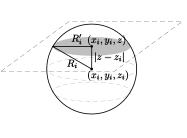
\includegraphics{fig/lnr_slice}
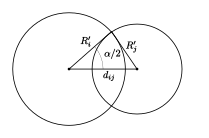
\includegraphics{fig/lnr_circles}
\caption{Geometry of slice in L\&R.\label{fig:slice}}
\end{figure}

The exposed arc lengths for each atom can be calculated exactly. For
each pair of atoms $i,j$, the distance between their centers projected
on the slice is $d_{ij}$ (independent of $z$). If $d_{ij} > R_i^\prime
+ R_j^\prime$, there is no overlap. If $d_{ij} < R_j^\prime -
R_i^\prime$ circle $i$ is completely inside $j$ (and the other way
around). If $d_{ij}$ lies between these two cases the angle of circle
$i$ that is buried due to circle $j$ is 
\begin{equation}
  \alpha = 2\arccos
  \bigl[({R_i^\prime}^2_{\,} + d_{ij}^2 - {R_{j}^\prime}^2_{\,})/(2R_i^\prime
  d_{ij})\bigr].
\end{equation}
If the middle point of this arc on the circle is at an angle $\beta$,
the arc spans the interval $[\beta-\alpha/2,\beta+\alpha/2]$. By
adding up these arcs and taking into account any overlap between them
we get the total buried angle $\gamma$ in this slices. The exposed
arc angle for this atom and slice is thus $2\pi-\gamma$ and the
total SASA of that atom
\begin{equation}\label{eq:LR_SASA}
  A_i =R_i \delta \sum_{s\in\text{slices}}
    \left[2\pi-\gamma_s\right]\,.
\end{equation}
The angle is multiplied by $R_i$ (not $R_i^\prime$) to give the area
of a conical frustum circumscribing the sphere at the slice. Finally,
the total area $A$ is the sum of all $A_i$.

In FreeSASA, the L\&R SASA calculation begins by finding overlapping
spheres and storing the contacts in an adjacency list. It then
iterates through all the slices of each atom and checks for overlap
with adjacent atoms in each slice, and adds up the exposed arcs to
calculate the atom's contribution to the SASA of the slice. The
calculations for each atom are completely independent and can thus be
parallelized over an arbitrary number of threads, whereas the
calculation of adjacency lists has not been parallelized.

\subsection{S\&R}

Shrake \& Rupley's algorithm uses test points on a sphere to estimate
what parts of an atom are exposed. Test points are generated on the
fly as a fibonacci grid~\cite{FibonacciGrid}.  For each atom $i$, use
a set of test points evenly distributed (approximately) over the
sphere of radius $R_i$, and count how many of the test points are not
inside any other sphere. The number of exposed test points divided by
the total number of test points gives the exposed solid angle of that
atom. The precision of the algorithm is increased by increasing the
number of test points, and calculation time scales approximately
linearly with the number of test points.  One potential speed-up of
this implementation, at least in the high accuracy limit, would be to
include a grid for the test points as well, as in the double cubic
lattice method~\cite{DCLM}.
 
\section{Performance and precision}\label{sec:performance}

To compare the computational efficiency of the two algorithms, the
most restrictive set of PDB files was downloaded from
PISCES~\cite{PISCES}.  88 PDB files were selected randomly from this
set by taking up to 10 structures (if available), in the sequence
length brackets $[0,100]$, $[100,200]$, $\dots$, $[1100,1200]$ amino
acids. The PISCES set specifies a specific chain in each file, but in
the following, all chains were used in each, which resulted in the
largest structure studied having over 30\,000 atoms (1JZ8). To average
out some variation in the running time in these rather short
calculations (in some cases 10's of milliseconds), each calculation was
run three times.

The calculation time of both algorithms scales linearly with the
number of atoms as can be seen from figure~\ref{fig:scaling}. The
effect of spreading the calculation over several threads can be seen
in figure~\ref{fig:threads}. Since the generation of Verlet lists is
not parallelized, using more than one thread only gives a significant
performance benefit at the limit of high precision. For the cases
studied here, using more than two threads only gives a limited
improvement~\cite{4cores}.
\begin{figure}
  \begin{center}
  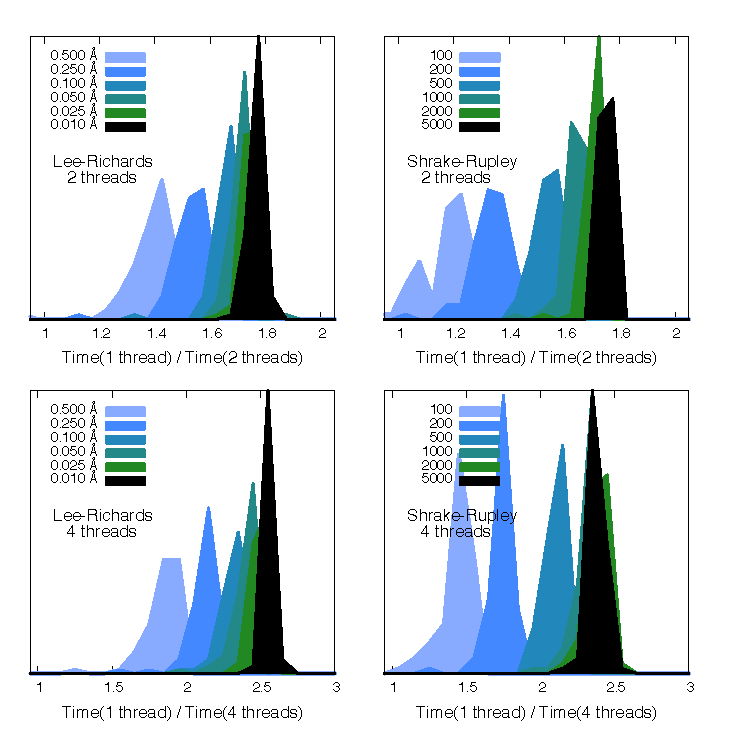
\includegraphics{fig/threads} 
  \caption{Comparison of calculation time with one, two and four
    threads, the histograms shows the distribution of the calculation
    time using two threads divided by the time using one thread. Thus
    values of two and four, respectively, would correspond to
    ``perfect'' parallelization.
    \label{fig:threads}}
  \end{center}
\end{figure}

To measure accuracy of the two algorithms a reference SASA value,
$S_\text{ref}$ was calculated using L\&R with slice thickness
$0.001\,\mathrm{\AA}$. The error of a given SASA-value, $S$ is then
$\epsilon = \lvert S - S_\text{ref} \rvert / N$, where $N$ is the
number of atoms in the protein. Figure~\ref{fig:precision} shows the
results of these calculations for the 88 proteins described above.

\begin{figure}
  \begin{center}
    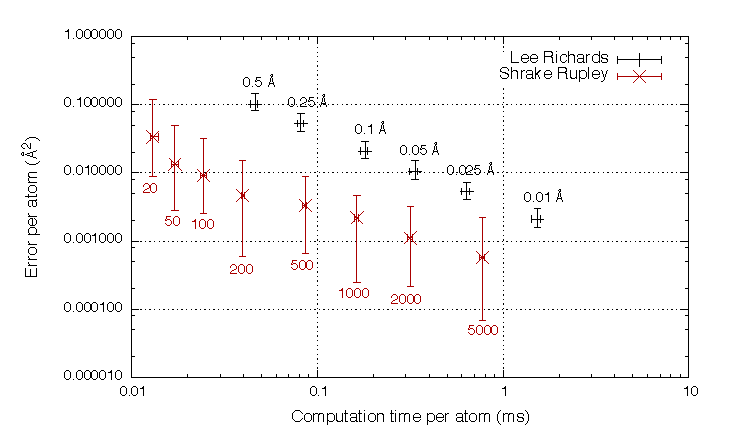
\includegraphics{fig/precision}
    \caption{The error $\epsilon$ in calculated SASA vs calculation
      time $t$ for the two algorithms and the programs POPS, NACCESS
      and DSSP. Labels indicate the precision used for each set of
      calculations (when available). The error bars indicate the 10th
      and 90th percentiles, i.e.\ $80\,\%$ of the values are within
      the error bars along both axes.  For the different S\&R
      calculations 20, 50, 100, 200, 500, 1000, 2000 and 5000 test
      points were used. For L\&R 5, 10, 20, 50, 100 and 200 slices per
      atom. A L\&R run with 1000 slices was used as reference to
      calculate the errors for both. The two points for POPS
      correspond to POPS-A and POPS-R, the large variation in
      computation time is because this algorithm is $O(N^2)$ in the
      number of atoms. NACCESS uses L\&R and was run with the three
      values of the z-parameter (0.1, 0.05 and 0.01, corresponding to
      10, 20 and 100 slices per atom~\cite{NACCESSParam}). A NACCESS
      run with z-parameter 0.005 was used as reference for both POPS
      and NACCESS. DSSP uses L\&R with 200 test points. SASA is only
      one of several calculations done by this program, explaining why
      it is significantly slower than FreeSASA with the same
      settings. FreeSASA L\&R with 1000 slices and the atomic radii
      taken from DSSP was used as reference to calculate errors here.
    \label{fig:precision}}
  \end{center}
\end{figure}

\begin{small}
  
\begin{thebibliography}{50}

\bibitem{GPL}
  See  \url{http://www.gnu.org/licenses/gpl.html}

\bibitem{LnR} 
  Lee B, Richards FM (1971) The interpretation of protein
  structures: estimation of static accessibility. Journal of molecular
  biology 55: 379--400.

\bibitem{NACCESS} 
  Hubbard SJ, Thornton JM (1993) NACCESS. Computer Program,
  Department of Biochemistry and Molecular Biology, University College
  London.

\bibitem{DSSP}
  Touw WG, Baakman C, Black J, et al. (2015)
  A series of PDB related databases for everyday needs.
  Nucleic Acids Research 43(Database issue): D364--D368.

\bibitem{SnR} 
  Shrake A, Rupley JA (1973) Environment and exposure to
  solvent of protein atoms. Lysozyme and insulin. Journal of Molecular
  Biology 79: 351--371.

\bibitem{DCLM}
  Eisenhaber F, Lijnzaad P, Argos P, Sander C, Scharf M (1994)
  The double cubic lattice method: efficient approaches to numerical
  integration of surface area and volume and to dot surface contouring
  molecular assemblies. Journal of Computational Chemistry 16: 273--284.

\bibitem{GetAreaURL}
  See \url{http://curie.utmb.edu/getarea.html}.

\bibitem{Getarea}
  Fraczkiewicz R, and Braun W, (1998) Exact and Efficient Analytical
  Calculation of the Accessible Surface Areas and Their Gradients for
  Macromolecules. Journal of Computation Chemistry 19: 319--333.

\bibitem{OONS} 
  Ooi T, Oobatake M, Némethy G, Scheraga H (1987)
  Accessible surface areas as a measure of the thermodynamic
  parameters of hydration of peptides. Proceedings of the National
  Academy of Sciences of the United States of America 84: 3086--3090.

\bibitem{Verlet} 
  Verlet L (1967). Computer ``Experiments'' on Classical
  Fluids. I. Thermodynamical Properties of Lennard-Jones
  Molecules. Physical Review 159: 98--103.

\bibitem{FibonacciGrid} Swinbank R, Purser JR (2006) Fibonacci grids:
  A novel approach to global modelling. Quarterly Journal of the Royal
  Meteorological Society 132: 1769--1793.

\bibitem{PISCES}
  Wang G, Dunbrack RL (2003) PISCES: a protein sequence culling server. 
  Bioinformatics 19:1589--1591.

\bibitem{4cores}
  The tests were run on a computer with four
  cores, so there was probably some performance lost due to
  interference from background process in the measurement with four
  threads.

\bibitem{NACCESSParam} The parameter $z$ in NACCESS is multiplied by
  the atomic diameter to get the slice width (i.e. $1/z$ gives the
  number of slices). The default $z=0.05$ thus gives a slice width of
  $0.28 - 0.32\,\mathrm{\AA}$ depending on the atom type.

\end{thebibliography}

\end{small}

\end{document}
